\documentclass{article}
\usepackage{graphicx}
\usepackage{caption}
\newcommand{\HRule}{\rule{\linewidth}{0.5mm}}

\begin{document}

\begin{titlepage}
\begin{center}
\textsc{\LARGE Team2 Inc.}\\[1.5cm]

% title
\HRule \\[1.4cm]
{ \huge \bfseries Ushahidi GeoRole Project Final Report}\\[0.4cm]

\HRule \\[1.5cm]

%Author Data
\begin{minipage}{0.4\textwidth}
\begin{center}
\large Michael Hnatiw, 1684988\\
\large Stephen Lind, 1735827\\
\large Taylor Parrish, 1616044\\
\end{center}
\end{minipage}

%bottom of page
\vfill
{\large \today}
\end{center}
\end{titlepage}

\section{Problem and Resolution}
\subsection{Introduction}
Our changes to Ushahidi implement the ``GeoRole'' functionality outlined in Heather's blog post based on a string matching technique. We envisioned GeoRoles as a method to restrict user reports and administrator verification in order to add credibility and specialization to Ushahidi reports. This system required modification to a variety of controllers, views and models as well as localization modification. The program is ready for a version 1.0 release as all required functionality is present and stable, however there is room is stil room to improve the user experience in future releases.

\section{Accomplishments}
\subsection{Main Map}
\begin{minipage}{\linewidth}
  \centering
  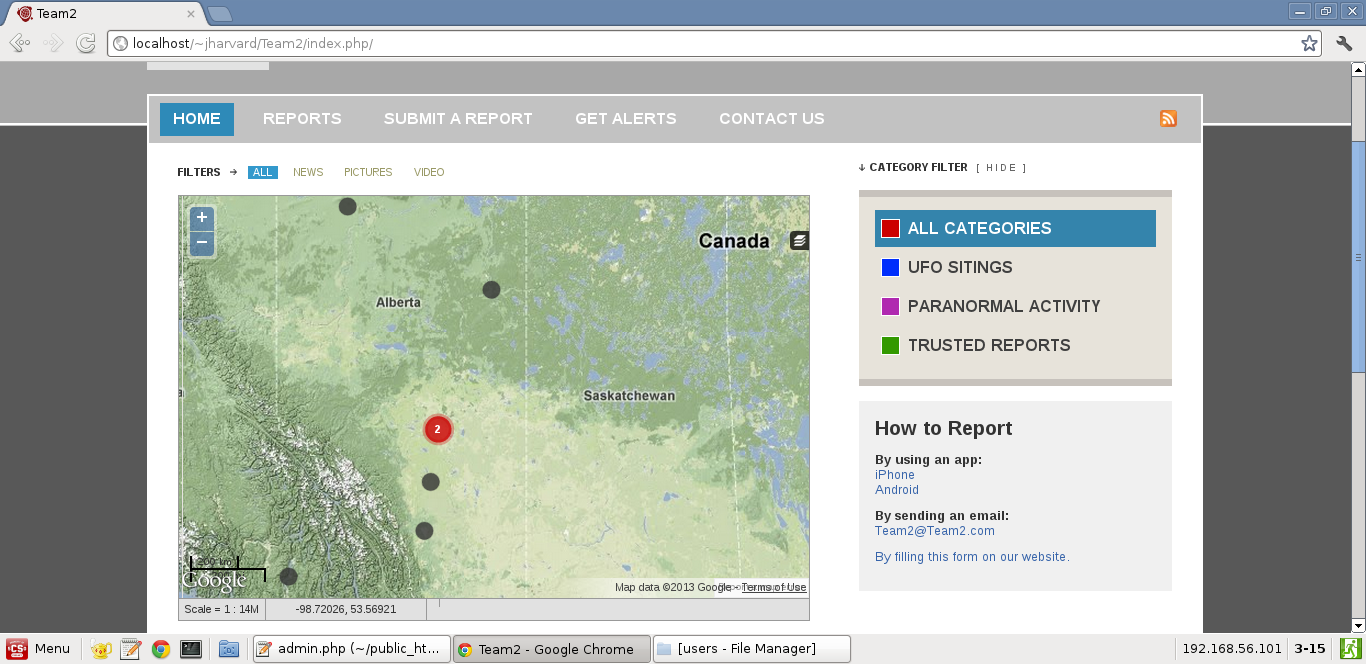
\includegraphics[width=100mm]{mainmapscreen.png}
  \captionof{figure}{Initial User View.}
\end{minipage}
The main map is filtered now based on GeoRole. If an incident on the map is within your GeoRole, the incident will show as red. If it is not, the incident will show as black. We manipulated jquery methods to implement this color change.

\subsection{Reports} 
\begin{minipage}{\linewidth}
  \centering
  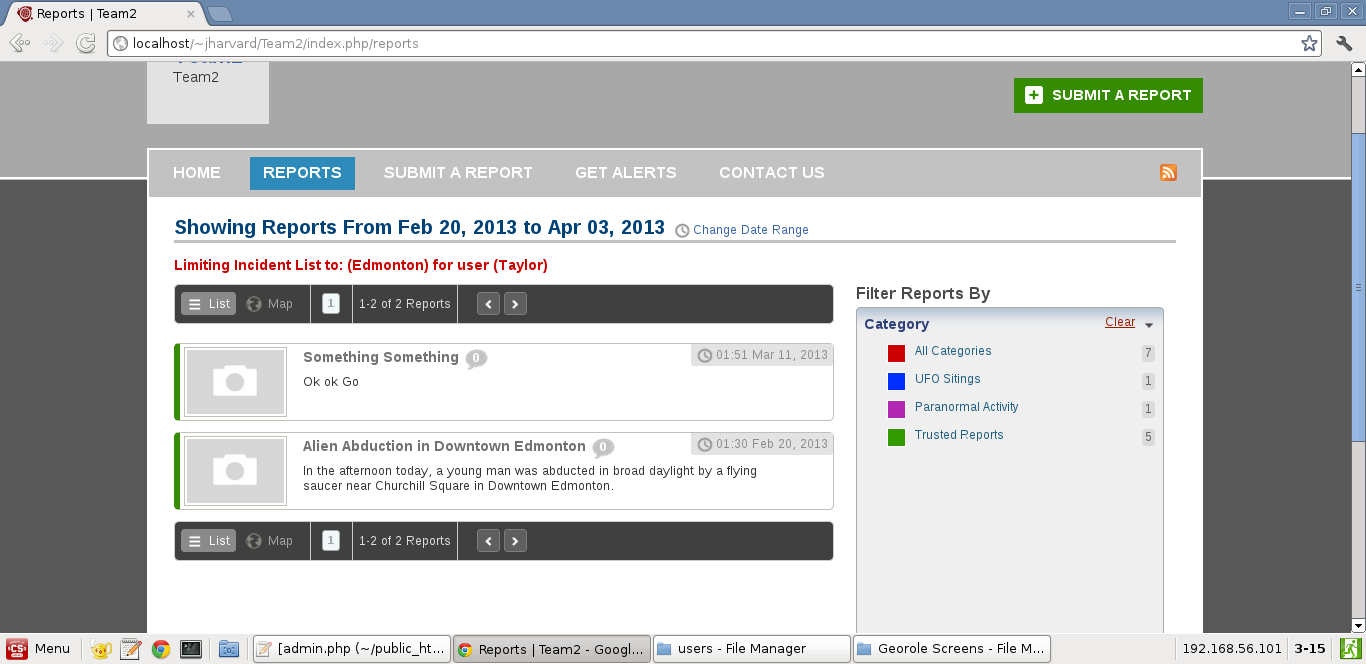
\includegraphics[width=100mm]{reports_list.png}
  \captionof{figure}{Filtered reports list.}
\end{minipage}
The report list is implicitly filtered by the user's GeoRole. If the user's GeoRole is not specified (ie. NULL) the Reports page will show all reports. This ensures that our version of Ushahidi is backwards compatible with the current official Ushahidi release.
\begin{itemize}
\item \subsection{Submission of Reports}
Admins implicitly cannot edit users outside of their GeoRole as they are not displayed in the view to the admin. The SuperAdmin is able to see all users and edit them at a global level.
\end{itemize}

\subsection{mySQL Database}
\begin{minipage}{\linewidth}
  \centering
  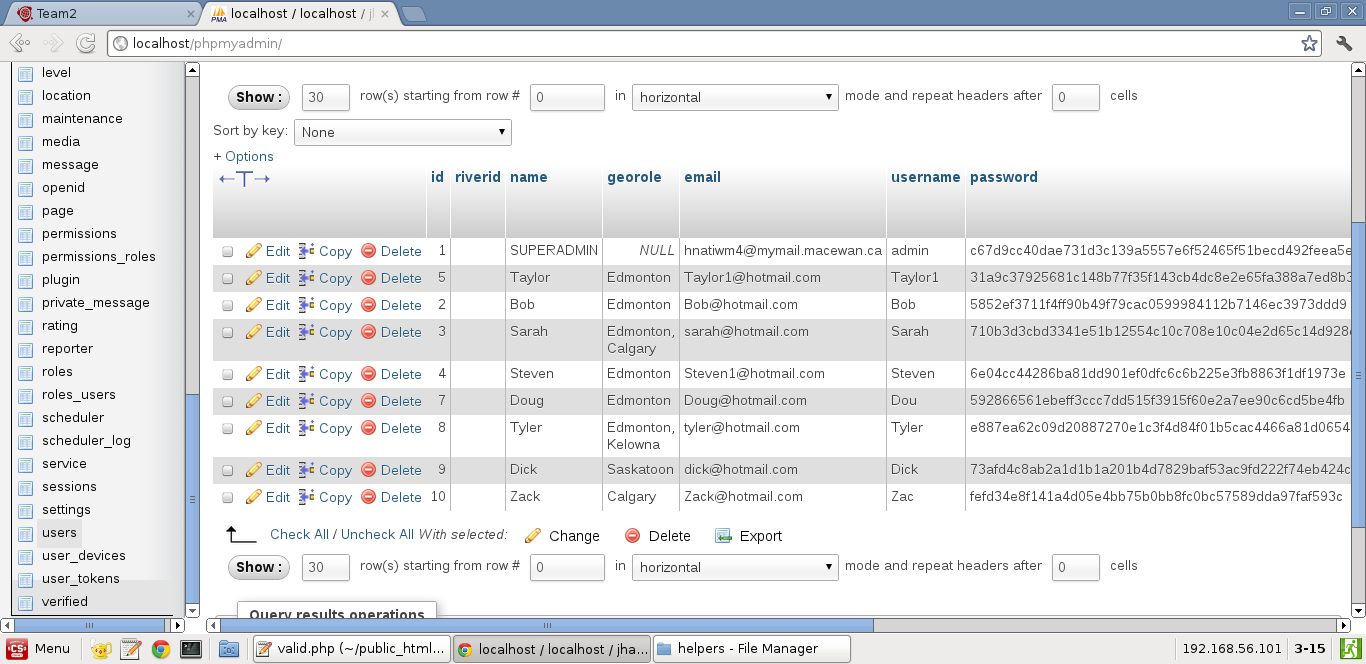
\includegraphics[width=100mm]{sql_table.png}
  \captionof{figure}{Database modifications.}
\end{minipage}
The SQL database was modified to contain a 100 character long field that is used to set GeoRole based on string comparison.

\section{Tools}
\subsection{JIRA Bug Tracking}
\begin{minipage}{\linewidth}
  \centering
  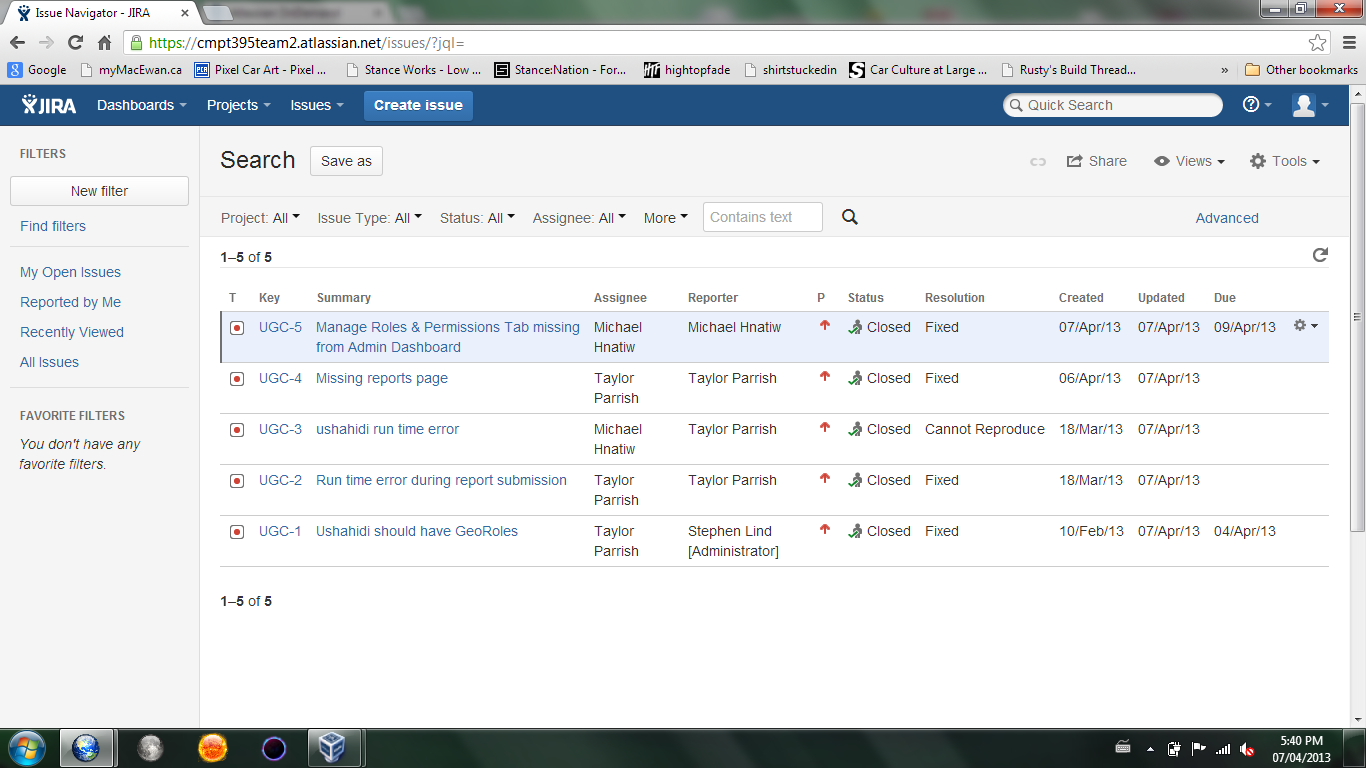
\includegraphics[width=100mm]{jira_bug_list.png}
  \captionof{figure}{Jira Bug List.}
\end{minipage}
We used Jira to track all of our bugs. Most of our bugs were short term and not filed, but anything that took more than a half hour or so was filed.
\subsection{GitHub}
GitHub was used as our version control. GitHub initially had a steep learning curve, but maintained a clean codebase. We eventually settled on branching from develop localy, then rebasing develop and merging the local branch as our general development procedure. We then merged with master on Mondays as a psuedo weekly build.

\section{Future Versions}
\subsection{Geometry Objects}
One of the project goals was to use a GUI based area selection using a polygon based tool. We were unable to implement this in the name of ensuring all base functionality and user hierarchy. This is the obvious next step for the next version release.
\subsection{Installation Procedure}
Currently the database has to be manually altered to add a GeoRole field under the ``User'' relation. THis should be set up at install time. Also we would like to implement an installation option for including GeoRoles.
\subsection{Abstraction of Package}
Coupled with the Installation procedure, we would like to abstract all of our work into a seperate package in the name of maintanability and object abstraction. This would clean up our work and ease integration with the main Ushahidi development branch.

\section{Development History}

\vfill
\begin{center}
Project Summary created with la\TeX~.
\end{center}
\end{document}
